\chapter{Implementierung}
\printmyminitoc{1}

\section{Umsetzung des Rogue Device}
Wie vorher schon beschrieben, wird ein Raspberry Pi 5 als Rogue Device benutzt. 
Als Betriebssystem wird Raspberry Pi OS benutzt. Dieses Betriebssystem ist eine auf Debian basierende Distribution, 
die speziell für den Raspberry Pi entwickelt wurde. Da der Raspberry Pi mit Linux betrieben wird, ist es die Bedienung
vergleichbar mit einem normalen Linux-System. Der Standard Package Manager ist apt. Unter dessen Benutzung werden 
Python 3.12 und die benötigten Bibliotheken installiert. Damit sind die Vorraussetzungen für die weitere Implementierung
gesetzt.


\section{Verbindung Rogue Device - Controller}
\begin{itemize}
    \item benutzt wird Python 3.12.8, da einfache Syntax und gute Bibliotheken
    \item Bibliothek: Pygame für die Controllereingabe (https://www.pygame.org/docs/(abgerufen am 08.12.2024))
    \item Beispielscode für Pygame: \href{https://github.com/kevinmcaleer/xbox_controller}{github} (abgerufen am 08.12.2024)
\end{itemize}

Im ersten Schritt wird der Controller mit dem Raspberry Pi verbunden. Der Raspberry Pi wird mit Raspberry Pi OS betrieben. 
Dieses Betriebssystem ist eine auf Debian basierende Distribution, die speziell für den Raspberry Pi entwickelt wurde.
Als Standard-Bluetooth-Treiber wird \href{https://www.bluez.org/}{BlueZ} verwendet. Dieser ist bereits vorinstalliert und muss 
nicht extra installiert werden. Da es sich in diesem Fall um einen XBox Controllers handelt, müssen die richtigen Treiber
(\href{https://github.com/xboxdrv/xboxdrv}{xboxdrv}) installiert werden. Diese können im apt-Repository gefunden werden.
Zusätzlich muss der Enhanced Re-Transmission Mode (ERTM) deaktiviert werden. Dieser Modus ist standardmäßig aktiviert und
verhindert die korrekte Verbindung des Controllers. Zum Schluss soll der Controller auf die aktuelle Firmware geupdatet werden.
Dies kann über die Xbox Accessories App gemacht werden, allerdings ist dies nur auf Windows möglich. Nun kann 
der Controller mit dem Raspberry Pi verbunden werden. Dies geschieht über die Bluetooth-Einstellungen des Raspberry Pi.
Um die Verbindung zu testen, kann eine Webapplikation benutzt werden. Diese zeigt die Eingaben des Controllers an. Zum 
Beispiel: \href{https://hardwaretester.com/gamepad}{hardwaretester} (abgerufen am 02.01.2025) 
\\
Als Programmiersprache wird Python 3 benutzt. Dies ist eine einfache Sprache, die viele Bibliotheken hat. Für die
Controller-Eingaben wird die Bibliothek Pygame benutzt. Diese Bibliothek ist einfach zu benutzen und hat viele Funktionen.
Sobald der Controller mit dem Raspberry Pi verbunden ist, wird dieser von Pygame erkannt. Die Eingaben des Controllers
können dann in Variablen gespeichert werden. Dabei gilt es zu beachten, dass der Gashebel oder die Ruderposition nicht
zu schnell verändert werden. Dies könnte zu unerwünschten Ergebnissen führen. Daher werden diese Werte mit Tasten des
Controllers eingegeben, welche nicht nur eine binäre Eingabe haben. Diese werden als Achsen bezeichnet. Diese ermöglichen
eine stufenlose Eingabe. Bei einer vollständigen Eingabe soll die Gashebelposition nach 20 Sekunden 100\% erreichen.
So ist sichergestellt, dass die Gashebelposition nicht zu schnell verändert wird. Die Ruderposition soll nach 2 Sekunden
in jede Richtung jeweils 100\% erreichen. Dies ist ein Kompromiss zwischen Geschwindigkeit und Genauigkeit.


Benutzte Hardware, Protokolle, Libraries 

\section{Übersetzung Signale Controller - Schiff}

Es gibt zuerst ein Programm, welches die Signale des Controllers erhält und in passende Variablen in Python interpretiert. Diese Variablen müssen
dann in Nachrichten für den Can-Bus umgewandelt werden. Hierfür gibt es ein weiteres Programm. Damit die beiden Programme miteinander kommunizieren
können, wird Inter-Process-Communication (IPC) benutzt. Als Methode werden hierbei Pipes benutzt. Diese sind einfach zu implementieren und haben
eine automatische Synchronisierung zwischen den Prozessen. Das bedeutet, dass die Prozesse nicht aufeinander warten müssen, sondern einfach
weiterarbeiten können. Es wird durch den Puffer der Pipe sichergestellt. Wenn dieser voll ist, wird der schreibende Prozess angehalten, bis der
lesende Prozess den Puffer geleert hat. Dies ist ein einfaches und effizientes Verfahren, 
um die beiden Prozesse zu synchronisieren \cite{Venkataraman2015}. 

\subsection{CAN-Bus}
Die Übertragenen Eingabewerte werden in dem nächsten Programm \texttt{canInterpreter.py} erkannt. Basierend auf den
Eingaben wird dann die entsprechende Nachricht erstellt. Um eine Nachricht zu kodieren, wird die Bibliothek \texttt{cantools} benutzt.
Mit dieser Bibliothek können DBC-Dateien gelesen und Nachrichten erstellt werden. Mit einer solchen Datei kann eine
bestimmte Nachricht mit ihren Signalen definiert werden. Es ist dafür notwendig, diese DBC-Datei zu verstehen.
\begin{figure}[H]
    \centering
    \includegraphics[scale=0.2]{images/CAN-DBC-File-Format-Explained-Intro-Basics_2.png}
    \caption{Auszug aus einer Beispiel DBC-Datei \cite{cssElectronics}(letzter Zugriff: 18.02.2025)}
    \label{fig:dbcfile}
\end{figure}

In dieser sind einzelne Nachrichten aufgelistet. Jede Nachricht hat eine ID, eine Länge und Signale. Diese Signale
haben eine Länge, einen Offset und einen Faktor. Mit diesen Informationen kann eine Nachricht erstellt werden.
Im Anschluss an die Nachrichtentypen werden in der DBC-Datei für bestimmte Signale die möglichen Eingaben definiert.
Das hilft bei der richtigen Wahl der Eingabe. \\
In der benötigten Nachricht ist eine Prüfsumme von 4 Bit notwendig. Jedoch gibt es zwei Methoden der Prüfsummenberechnung
nach dem SAE J1939 Standard \cite{VectorSAE} (letzter Zugriff: 18.02.2025). Die richtige Methode für das System der 
Limanda wurde durch aufgezeichnete Nachrichten ermittelt. Am Ende wird die Prüfsumme der Nachricht hinzugefügt und die
Nachricht wird an den Can-Bus gesendet. \\
Zusätzlich hilft das Programm \texttt{canReader.py} bei der Überwachung des Can-Bus. Es kann die Nachrichten auf dem
Can-Bus lesen und in Echtzeit dekodieren. Dazu wurde wieder die Bibliothek \texttt{cantools} benutzt. Auch hier wird
mit der gleichen DBC-Datei gearbeitet, da es sich um die gleichen Nachrichten handelt. In den dekodierten Nachrichten
können die Signale und deren Werte gesehen werden. Dies hilft bei der Überwachung des Systems. Es wird spezifisch nach
dem Signal für die Gashebelposition gesucht. Wenn dieses Signal entdeckt wird, dann muss eine eigene Nachricht
gesendet werden, um die wahren Eingaben zu verhindern. Dies passiert wieder durch \texttt{canInterpreter.py} nach 
einem über Pipes übermittelten Signal.  \\

\subsection{Serielle Schnittstelle}

\subsection{Eingabe-Interface}
Durch die begrenzte Zeit dieser Arbeit, wurde die Rückmeldung mit Vibrationen im Xbox-Controller implementiert.
Dabei wird bei Erreichen des Maximums oder Minimums der Gashebelposition eine Vibration ausgelöst. Dies ist eine einfache
Methode, um dem Benutzer eine Rückmeldung zu geben. Auch bei der hälfte der Gashebelposition wird eine kurze und leichte 
Vibration ausgelöst. Das soll ermöglichen, dass es eine ungefähre Vorstellung der Gashebelposition gibt.
Bei der Ruderposition wird eine Vibration ausgelöst, wenn die Ruderposition 100\% erreicht hat in jeweils beide Richtungen
erreicht hat. Bei der Mitte der Ruderposition wird eine kurze und leichte Vibration ausgelöst. Wenn die 
Ruderposition auf 50\% in eine Richtung ist, werden zwei kurze und leichte Vibrationen ausgelöst. Dies soll die Bedienung
erleichtern. Zusätzlich soll der Effekt von \textcolor{red}{pilot induced oscillation} verhindert werden. Dies ist ein Effekt,
bei dem der Pilot zu stark gegensteuert und somit eine Schwingung entsteht. Dafür muss der Schiffsführer 
die ungefähre Position des Ruders kennen. Dies wird durch die Vibrationen erreicht.\\
\\
Die Ruderstellung wird durch den linken Stick des Controllers gesteuert. Wenn die Eingabe eine bestimmte Schwelle überschreitet,
wird dies wie Folgt durch Vibrationen signalisiert:
\begin{figure}[h!]
    \centering
    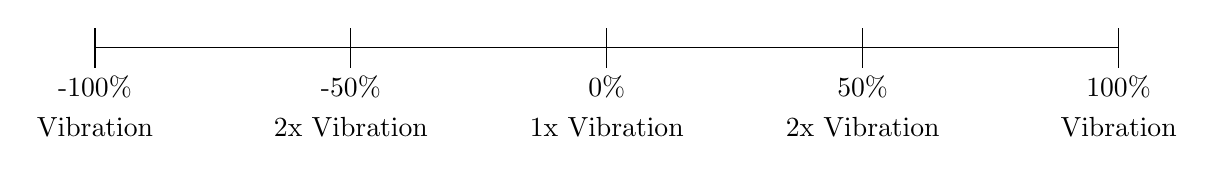
\begin{tikzpicture}
        \draw (0,0) -- (13,0);
        \draw (0,0.25) -- (0,-0.25);
        \draw (0,-0.5) node {-100\%};
        \draw (0,-1) node {Vibration};
        \draw (3.25, 0.25) -- (3.25, -0.25);
        \draw (3.25,-0.5) node {-50\%};
        \draw (3.25,-1) node {2x Vibration};
        \draw (6.5,0.25) -- (6.5,-0.25);
        \draw (6.5,-0.5) node {0\%};
        \draw (6.5,-1) node {1x Vibration};
        \draw (9.75,0.25) -- (9.75,-0.25);
        \draw (9.75,-0.5) node {50\%};
        \draw (9.75,-1) node {2x Vibration};
        \draw (13,0.25) -- (13,-0.25);
        \draw (13,-0.5) node {100\%};
        \draw (13,-1) node {Vibration};
    \end{tikzpicture}
\end{figure}
Dabei ist die Schwelle so gewählt, dass die Vibrationen nicht zu oft ausgelöst werden. 
Es ist wichtig zu wissen, dass der Wert basierend auf der Eingabe des Joysticks kontinuierlich berechnet wird.
Die Eingabe beträgt -1 bis 1. Dabei ist -1 die maximale Position nach links und 1 die maximale Position nach rechts.
Damit die Ruderstellung nicht zu schnell verändert wird, benötigt es eine volle Eingabe von 1 oder -1 für 2 Sekunden,
damit die Ruderstellung 100\% erreicht. Entsprechend werden diese 100\% langsamer erreicht, wenn die Eingabe geringer
ist.
